% !TeX spellcheck = en_US
\section{Magnetic properties}

\subsection{Magnetic moments\buch{685}}
The magnetic dipole moment is
\begin{equation}
    \vec{\mu_m} = I A \vec{u_n} = I \pi a^2 \vec{u_n}
\end{equation}

This creates a magnetic field $B$
\begin{equation}
    B = \frac{2 \mu_0 \mu_m}{4 \pi (r^2 + a^2)^{3/2}}
\end{equation}

A magnetic dipole placed in an external field $B$ experiences a \emph{torque}
which tries to align the dipole axis with the magnetic field.

\subsubsection{Orbiting electron}
\begin{figure}[ht!]
    \centering
    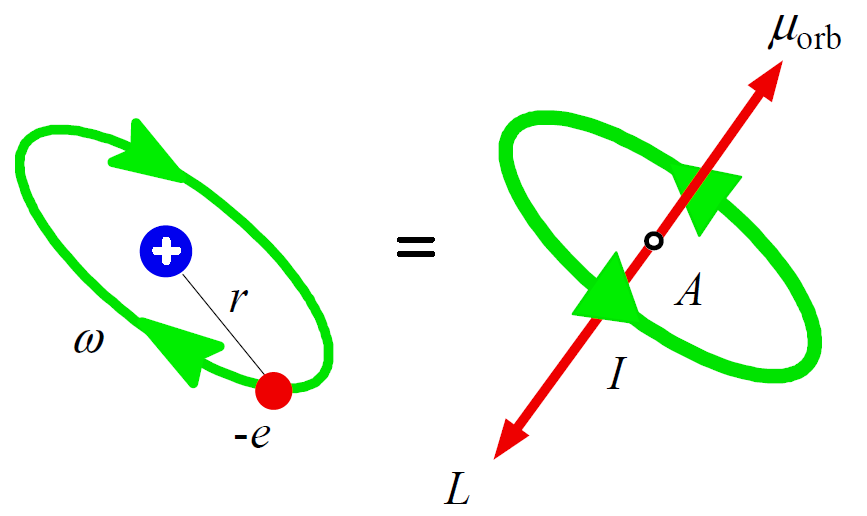
\includegraphics[width=0.4\linewidth]{images/orbiting_e.png}
    \caption{Orbiting electron in an atom}
\end{figure}

An orbiting electron in an atom behaves like a current loop
\begin{equation}
    I = -\frac{e}{T} = - \frac{e \omega}{2 \pi}
\end{equation}
and creates an orbital magnetic moment
\begin{equation}
    \mu_{orb} = I(\pi r^2) = -\frac{e \omega r^2}{2} = -\frac{e}{2 m_e} L
\end{equation}
where $L$ is the angular momentum
\begin{equation}
    L = (m_e v)r = m_e \omega r^2
\end{equation}
and the gyromagnetic ratio is $e / 2m_e$.

\subsubsection{Electron spin}
The electron spin also creates a magnetic dipole moment
\begin{equation}
    \mu_{spin} = -\frac{e}{m_e}S
\end{equation}
which is by a factor 2 greater.

with 
\begin{equation}
S_z = \pm \frac{1}{2} \hbar
\end{equation}
the spin dipole moment becomes
\begin{equation}
    \mu_z = -\frac{e \hbar}{2 m_e}
\end{equation}

\paragraph{Bohr magneton}
A single electron spin has the magnetic momentum of 1 Bohr magneton along the field.
\begin{equation}
    \beta = \frac{e \hbar}{2 m_e} = \SI{9.27e-24}{\ampere\square\meter}
\end{equation}

The magnitude of the electron spin is 
\begin{equation}
    S = \hbar \sqrt{s (s+1)} \underset{s=1/2}{=} \frac{\sqrt{3}}{2} \hbar
\end{equation}

\paragraph{Total angular momentum}
The total angular momentum is then
\begin{equation}
    \vec{J} = \vec{L} + \vec{S}
\end{equation}
Only \emph{unfilled} subshells contribute to the overall magnetic moment.
An atom with a single electron in an s orbital only has a spin momentum.

\subsection{Magnetization Vector}
For a coil with vacuum inside, the magnetic field is
\begin{equation}
    B_0 = \mu_0 \frac{N I}{l} = \mu_0 I'
\end{equation}
where $I' = \frac{NI}{l}$ is the current per length.

For a coil with material inside, each atom acquires a magnetic moment $\mu_0$ along the field $B_0$.
The magnetic dipole moment per unit volume is
\begin{equation}
    \vec{M} = \frac{1}{V} \sum\limits_{i=1}{N}\vec{\mu}_{mi} = n_{atom} \vec{\mu}_{av}
\end{equation}

Each atomic magnet moment can be viewed as current loop.
The current loops add up to a net surface current, induced by
the magnetization of the medium.
\begin{equation}
    \mu_{tot} = MAl = (I_m l) A = M \times \text{volume} = \text{Current} \times \text{Area}
\end{equation}
where $I_m = M$ is the magnetization current per unit length.

The magnetic field is then
\begin{align}
    B &= \mu_0 (I' + I_m) \\
    \vec{B} &= \vec{B}_0 + \mu_0 \vec{M}
\end{align}

The magnetic intensity field is
\begin{equation}
    \vec{H} = \frac{1}{\mu_0}\vec{B}_0 = \frac{1}{\mu_0}\vec{B} - \vec{M}
\end{equation}
$H$ can also be viewed as cause for $B$:
\begin{equation}
    H = \frac{N I}{l} ) I'
\end{equation}

\subsection{Magnetic permeability and susceptibility}
The magnetic permeability relates the effect $B$ to the cause $H$
\begin{equation}
    \mu = \frac{B}{H} = \mu_0 \mu_r
\end{equation}
with the relative permeability of a medium
\begin{equation}
    \mu_r = \frac{B}{B_0} = \frac{B}{\mu_0 H}
\end{equation}

The magnetic susceptibility $\chi_m$ of the medium relates
\begin{equation}
    \vec{M} = \chi_m \vec{H}
\end{equation}
so
\begin{equation}
    \mu_r = 1 + \chi_m
\end{equation}

\begin{table}[ht!]
    \centering
    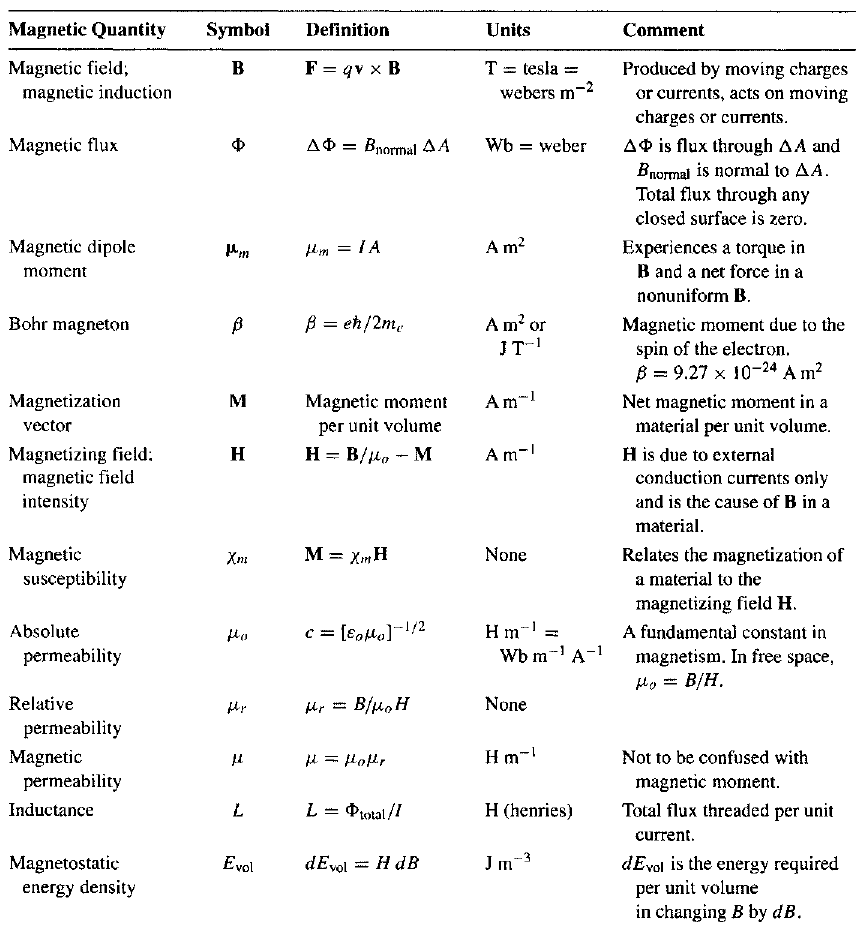
\includegraphics[width=0.8\linewidth]{images/magnet_formulas.png}
    \caption{Definitions and units of magnetic quantities.}
\end{table}

\subsection{Magnetic material classifications\buch{696}}
\subsubsection{Diamagnetism\buch{696}}
\subsubsection{Paramagnetism\buch{698}}
\subsubsection{Ferromagnetism\buch{699}}
\subsubsection{Antiferromagnetism\buch{699}}
\subsubsection{Ferrimagnetism\buch{700}}

\subsection{Saturation magnetization and Curie temperature\buch{703}}
The Curie temperature $T_C$ is the critical temperature at which ferromagnetic behavior is lost

\begin{align*}
    T < T_C \qquad &\text{Ferromagnetism} \\
    T > T_C \qquad & \text{Paramagnetism}
\end{align*}
The energy of exchange interaction is responsible for spin alignment:
$ E_{ex} \approx k T_C \approx \SI{0.1}{\electronvolt}$.

\subsection{Magnetic domains\buch{705}}
\subsubsection{Magnetostriction\buch{711}}
A magnetic field along the easy direction causes an elongation along 
the easy direction and a contraction in traverse directions.
The magnetostrictive constant corresponds to the longitudinal strain
\begin{equation}
    \lambda = \frac{\Delta l}{l}
\end{equation}

\subsection{Giant magnetoresistance (GMR)\buch{744}}
The giant magnetoresistive effect is caused by ferromagnetic layer
separated by non-magnetic conducting layers.
The layers need to be smaller than the electron mean free path (few nm)

